%%%%%%%%%%%%%%%%%%%%%%%%%%%%%%%%%%%%%%%%%
% Beamer Presentation
% LaTeX Template
% Version 1.0 (10/11/12)
%
% This template has been downloaded from:
% http://www.LaTeXTemplates.com
%
% License:
% CC BY-NC-SA 3.0 (http://creativecommons.org/licenses/by-nc-sa/3.0/)
%
%%%%%%%%%%%%%%%%%%%%%%%%%%%%%%%%%%%%%%%%%

%----------------------------------------------------------------------------------------
%                                                                     PACKAGES AND THEMES
%----------------------------------------------------------------------------------------
\pdfminorversion=4
\documentclass{beamer}

\mode<presentation> {

%                                            The Beamer class comes with a number of
%                                            default slide themes which change the colors
%                                            and layouts of slides. Below this is a list
%                                            of all the themes, uncomment each in turn to
%                                            see what they look like.

%\usetheme{default}
%\usetheme{AnnArbor}
%\usetheme{Antibes}
%\usetheme{Bergen}
%\usetheme{Berkeley}
%\usetheme{Berlin}
%\usetheme{Boadilla}
%\usetheme{CambridgeUS}
%\usetheme{Copenhagen}
%\usetheme{Darmstadt}
%\usetheme{Dresden}
%\usetheme{Frankfurt}
%\usetheme{Goettingen}
%\usetheme{Hannover}
%\usetheme{Ilmenau}
%\usetheme{JuanLesPins}
%\usetheme{Luebeck}
\usetheme{Madrid}
%\usetheme{Malmoe}
%\usetheme{Marburg}
%\usetheme{Montpellier}
%\usetheme{PaloAlto}
%\usetheme{Pittsburgh}
%\usetheme{Rochester}
%\usetheme{Singapore}
%\usetheme{Szeged}
%\usetheme{Warsaw}

%                                            As well as themes, the Beamer class has a number
%                                            of color themes for any slide theme. Uncomment
%                                            each of these in turn to see how it changes the
%                                            colors of your current slide theme.

%\usecolortheme{albatross}
%\usecolortheme{beaver}
%\usecolortheme{beetle}
%\usecolortheme{crane}
%\usecolortheme{dolphin}
%\usecolortheme{dove}
%\usecolortheme{fly}
%\usecolortheme{lily}
%\usecolortheme{orchid}
%\usecolortheme{rose}
%\usecolortheme{seagull}
%\usecolortheme{seahorse}
%\usecolortheme{whale}
%\usecolortheme{wolverine}

%\setbeamertemplate{footline} %              To remove the footer line in all
%                                            slides uncomment this line
%\setbeamertemplate{footline}[page number] % To replace 
%                                            the footer line in all slides with a simple
%                                            slide count uncomment this line

%\setbeamertemplate{navigation symbols}{} %  To remove the
%                                            navigation symbols from the bottom of all 
%                                            slides uncomment this line
}

%----------------------------------------------------------------------------------------
%                                                                           Custom Colors
%----------------------------------------------------------------------------------------
\AtBeginSection{\frame{\sectionpage}}

\definecolor{UC_blue}{RGB}{18,149,216}

\setbeamercolor{structure}{fg=UC_blue}


\usepackage{graphicx} %                      Allows including images
\usepackage{booktabs} %                      Allows the use of \toprule, \midrule
%                                            and \bottomrule in tables

%----------------------------------------------------------------------------------------
%	                                                                       Title Page
%----------------------------------------------------------------------------------------

%                                            The short title appears at the bottom of
%                                            every slide, the title is only on the
%                                            title page
\title[Network Process Modeling]{Parameter Estimation for Networks Processes}

\author{Steven Munn} %                       Your name

%                                            Your institution as it will appear on the
%                                            bottom of every slide, may be shorthand to
%                                            save space
\institute[UCSB]
{
University of California, Santa Barbara \\ % Your institution for the title page
\medskip
\textit{sjmunn@umail.ucsb.edu} %             Your email address
}
\date{\today} %                              Date, can be changed to a custom date

\begin{document}

\begin{frame}
\titlepage %                                 Print the title page as the first slide
\end{frame}

\begin{frame}
\frametitle{Overview} %                      Table of contents slide, comment 
%                                            this block out to remove it
\tableofcontents %                           Throughout your presentation, if
%                                            you choose to use \section{} and
%                                            \subsection{} commands, these will
%                                            automatically be printed on this slide
%                                            as an overview of your presentation
\end{frame}

%----------------------------------------------------------------------------------------
%	                                                              Presentation Slides
%----------------------------------------------------------------------------------------

%------------------------------------------------
\section{Graph Attributes}

\begin{frame}
\frametitle{Attributed Graphs}
%                                            We are interested in representing problems
%                                            as graphs with attributes
\begin{figure}
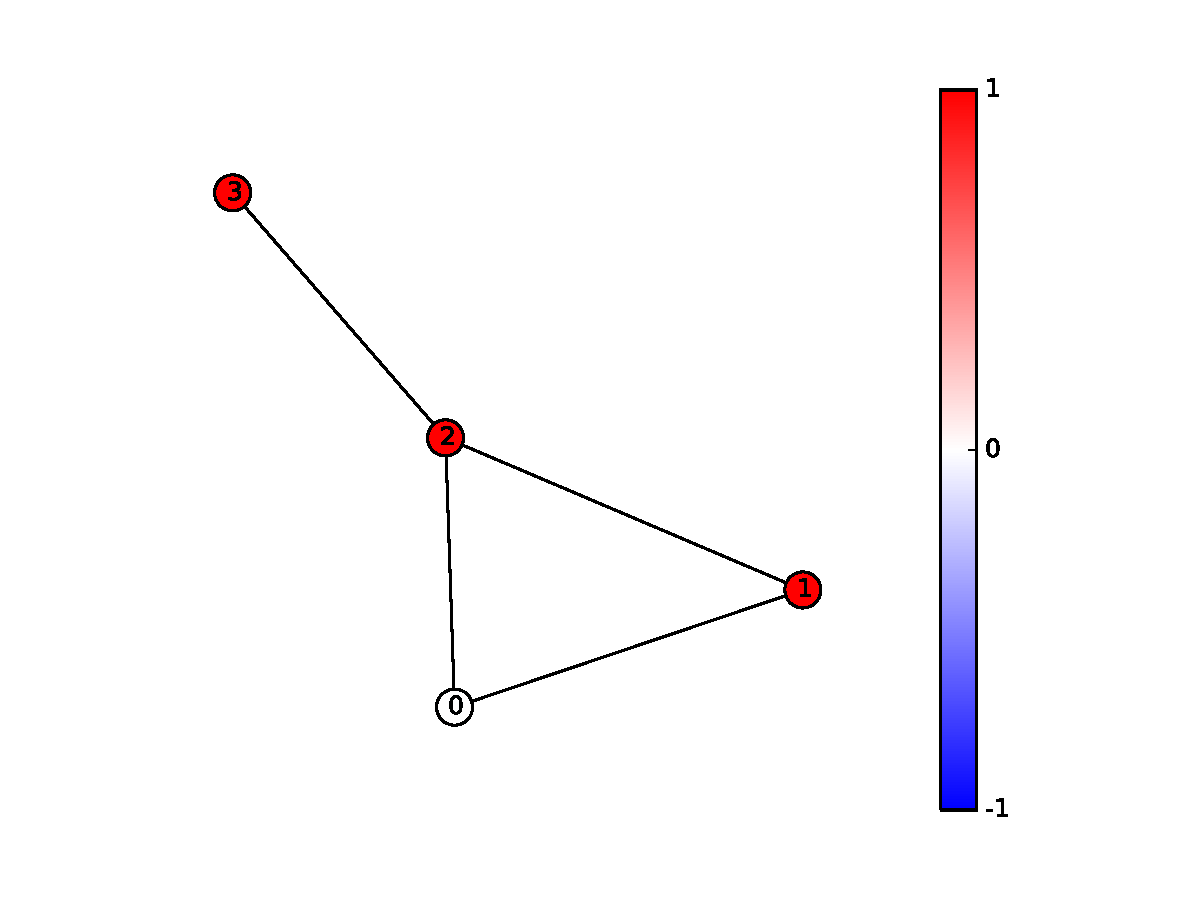
\includegraphics[width=0.8\linewidth]{figs/attributed_graph}
\end{figure}
\end{frame}

\begin{frame}
\frametitle{Traffic Example}
\begin{figure}
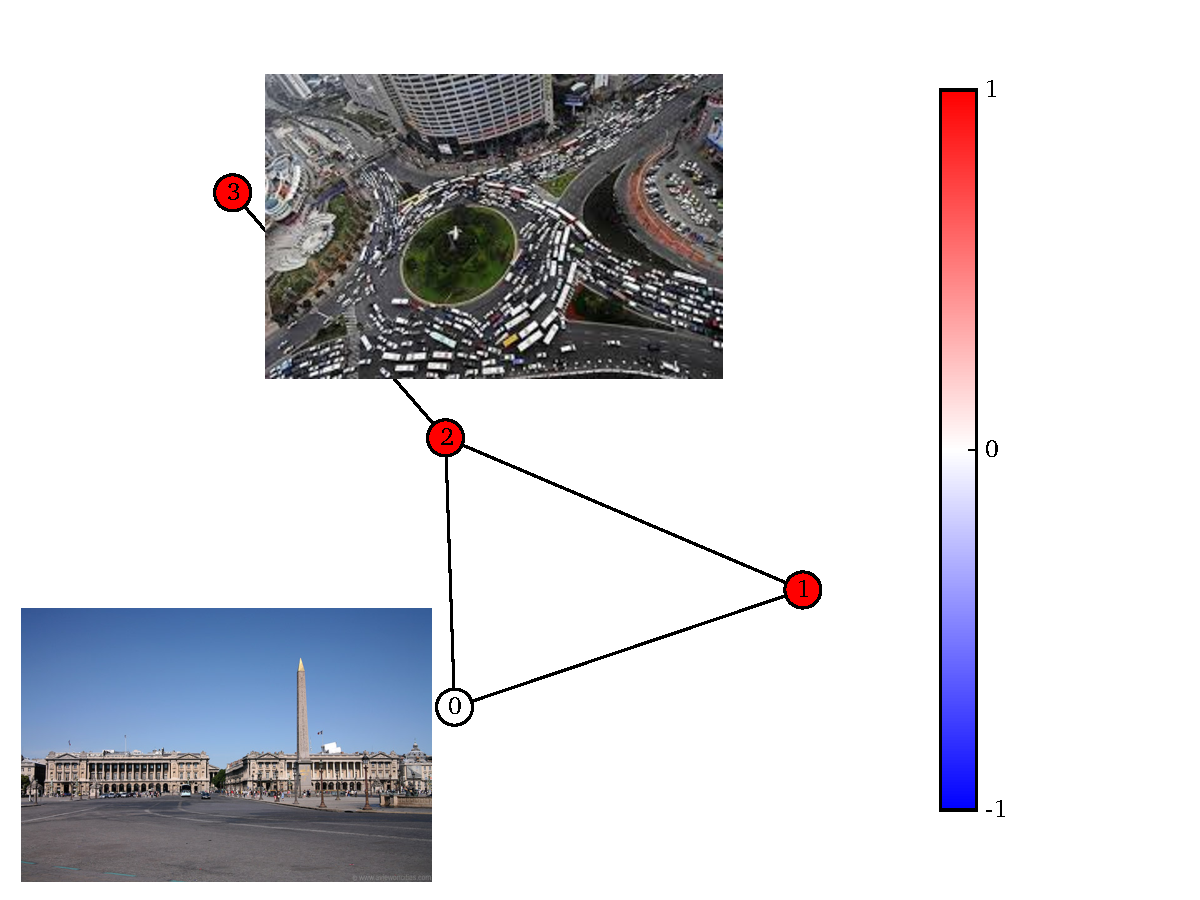
\includegraphics[width=0.8\linewidth]{figs/trafficEg}
\end{figure}
\end{frame}

\begin{frame}
\frametitle{Website Visits Example}
\begin{figure}
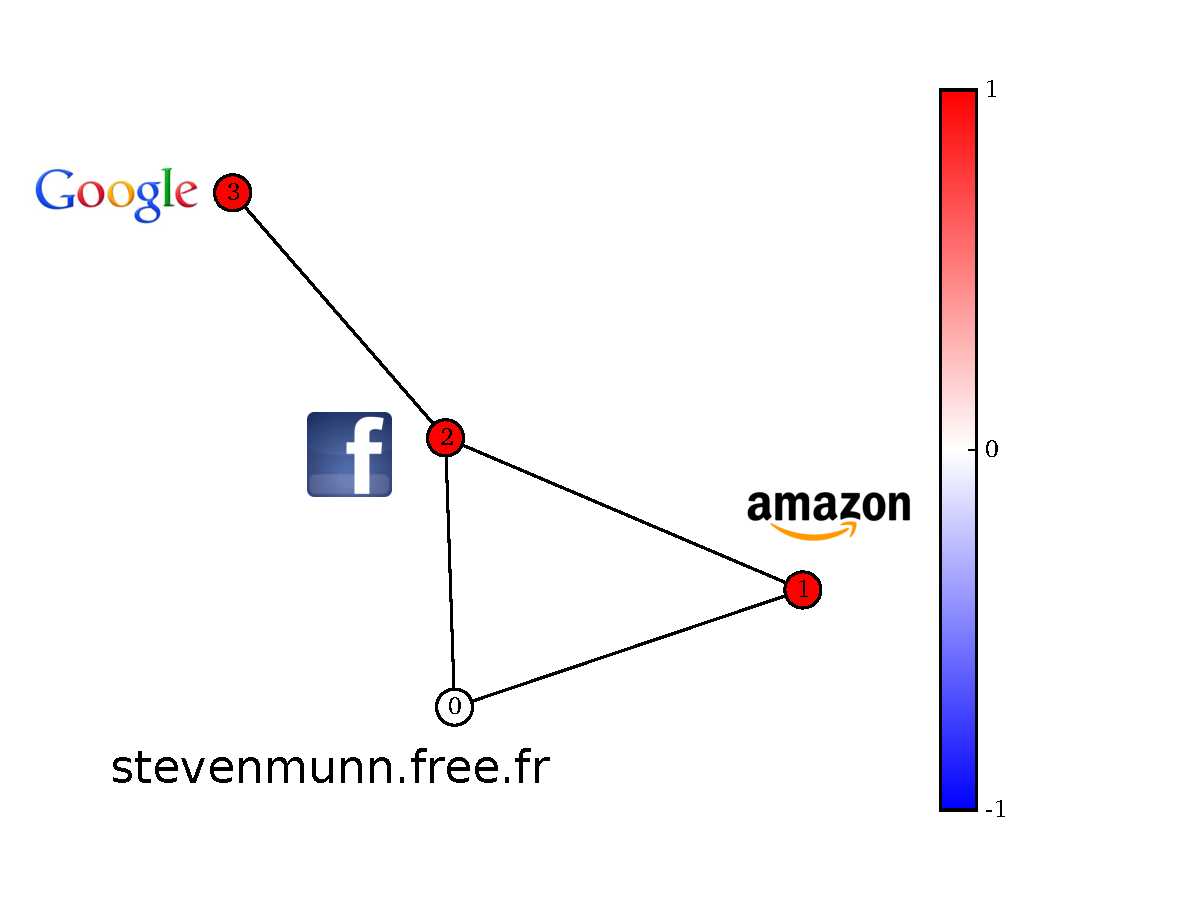
\includegraphics[width=0.8\linewidth]{figs/websitesEg}
\end{figure}
\end{frame}
%------------------------------------------------
\section{Reaction Networks}

\begin{frame}
\frametitle{Reaction Attributes}
\begin{figure}
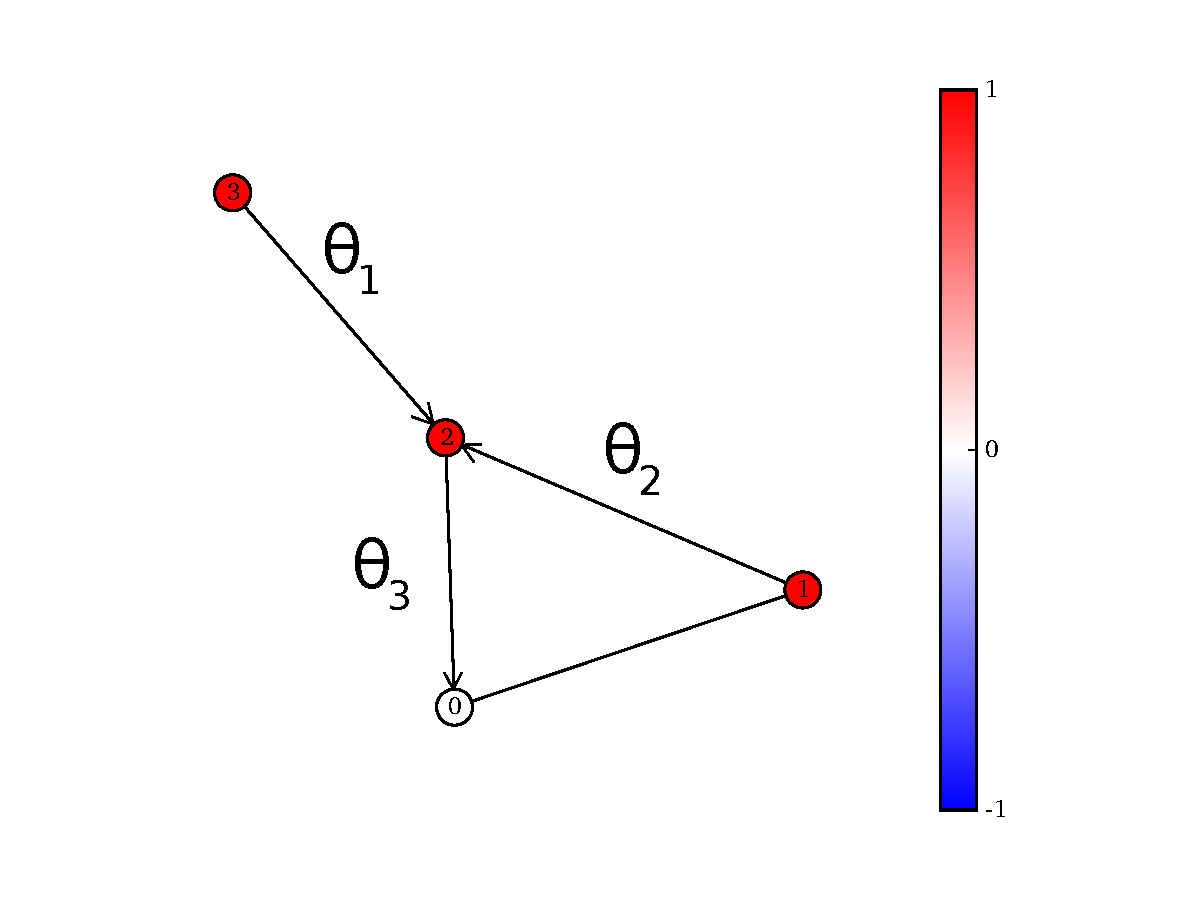
\includegraphics[width=0.8\linewidth]{figs/reaction_graph}
\end{figure}
\end{frame}

\begin{frame}
\frametitle{Estimate Parameters}
The goal is to model the process that creates the graph attributes.
\end{frame}

\end{document}